\section{Introduction}

% object model is critical
All data is presented as object in mainstream dynamic languages like Python, Ruby and JavaScript.
Programs written in those languages interact with data using objects.
Object model, the implementation behind the object representation is a core component of a language runtime implementation.
Not only it has to be efficient for accessing the reperesented data, it also needs to respect the dynamic nature of those languages.
An efficient dynamic language implementation should handled object modifications at runtime in less expensive ways.

% hosted language is the trend
Despite their popularity, performance has been the weakness of dynamic languages.
Languages like Python and Ruby are originally implemented as interpreters.
Although interpreters are easy to implement, their performance is suboptimal.
To address this weakness, we have seen previous works that have improved the performance of dynamic languages
by constructing a complete just-in-time (JIT) compilation based virtual machine for one particular language.
This approach offers promising performance benefit, but incurs significant implementation costs.

Alternatively, language implementors can build their languages on top of an existing mature virtual machine such as the Java Virtual machine (JVM).
In this way, the ``guest'' language can reuse the existing components of the ``hosting'' virtual machine to alleviate its implementation costs.
It also provide the opportunity for the ``hosted'' language to take advantage of the underlying JIT compiler to address its performance issue.
We explore the performance potential of ``hosted'' interpreters for dynamic languages.
We do so by hosting a ``highly dynamic'' language (Python) on the JVM, a VM for ``moderately dynamic'' languages.

% existing hosted object model has drawbacks
We found that existing hosted dynamic languages have not addressed their object model in an efficient way.
Jython, a JVM based Python implementation replicate the same object model design we saw in CPython to Java.
This approach failed to identify the strength of the underlying VM.
It relies on the assumption that the underlying JIT is powerful enough to optimize any type of program.
Truffle's object model framwork provided an efficient way for guest langauge developer to quickly build a performant object model.
It makes use of highly efficient constructs provided by the ``hosting'' VM.
However it's design uses a fixed object storage layout, which often trades space for performance.
In practice, this approach addes unnecessary pressure to the garbage collector when running programs allocates object frequently.

% our extension to that
In this paper, we propose an improved object model for hosted dynamic languages.
It addresses the performance and space drawbacks of the existing works.
We demonstrate our technique using our own full-fledged prototype implementation of Python 3, called ZipPy\footnote{Publicly available at \url{https://bitbucket.org/ssllab/zippy}}, which targets the Java virtual machine (JVM).
ZipPy uses the Truffle framework to optimize interpreted programs in stages, first collecting type feedback in the AST interpreter, then just-in-time compiling an AST down to optimized machine code.

\noindent{}Our contributions are:

\begin{itemize}

\item We present an efficient object model implementation for hosted dynamic languages.

\item We introduce \emph{flexible object layout evolution}, a new technique our system uses to minimize space overheads incurred by object model.

\item We provide results of a careful and detailed evaluation of our optimization and report:
  \begin{itemize}
  \item an average saving of xxx over the fixed storage baseline.
  \end{itemize}
\end{itemize}

\section{Background}

In Python all data is an object.
CPython, the original implementation of Python, constructs every data type in Python as a heap allocated data structure.
Since it is written in C, CPython implements Python built-in data types using C struct and user defined types using hash maps.
This model results in expensive arithmetic operations due to frequent accesses and allocations of data structures in the heap.
Hash map based object model is also inefficient.
Although the cost of hash map operations is amortized for large data sets, the overhead of retrieving or updating a single map entry is still expensive.
In a hash map based object model, retrieving the value of an object field, or an object attribute in Python, is equivalent to reading the value of a map entry.
This operation involves a hashing calculation and a few steps of memory accesses before reaching the memory address that stores the target value.
On the other hand, in a traditional programming language like Java, an object field access, if optimized, is simply a single memory read.
In summary, object model inefficiency is the main impediment to the performance of popular dynamic languages like Python.

\subsection{Jython's Object Model Design}

Existing JVM based Python implementations like Jython, however, replicate the same object model design we saw in CPython.
The main approach they took is porting the existing design from C to Java hoping that the underlying Java compiler will magically optimize it.
This approach failed to realize that, although, the Java JIT compiler is powerful, its strength is in compiling and optimizing programs written in Java,
the first class citizen of the JVM.
Hence, without additional knowledge to the guest language, the Java compiler is unable to address the miss match between the object model of the guest language and Java in an efficient way.
A more efficient solution requires identifying the strengths of the Java compiler and mapping critical components of the guest language onto efficient constructs offered of the JVM.
In the rest of this Section, we describe how we close the gap between the object models of Python and the JVM in ZipPy.

\subsection{Python on Truffle}

\begin{figure*}[!ht]
\centering
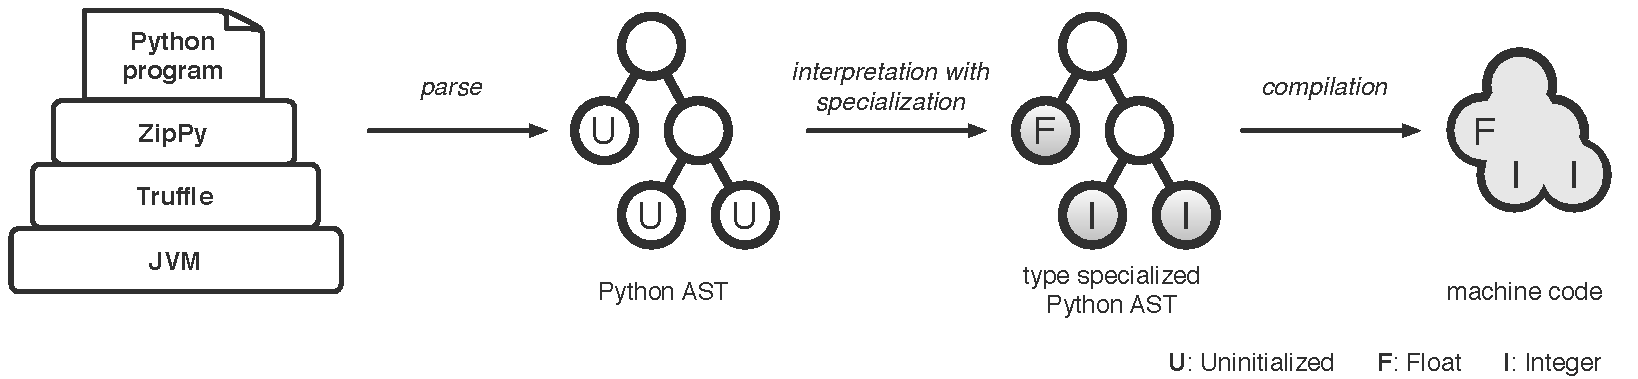
\includegraphics[scale=0.50]{figures/python-on-truffle.pdf}
\caption{Python on Truffle}
\label{fig:python_on_truffle}
\end{figure*}

In principle, ``everything'' can change at any moment in dynamic language programs.
This dynamic nature is the major impediment to ahead-of-time optimization.
In practice, however, programmers tend to minimize the rate of change, which makes the code highly predictable.
Types, for instance, typically remain stable between successive executions of a particular operation instance.
Deutsch and Schiffman report that speculative type specialization succeeds 95\% of the time in their classic Smalltalk-80 implementation~\cite{Deutsch1984}.

Truffle is a self-optimizing runtime system that makes it easy to perform type specialization for dynamic languages running on top of the Java Virtual Machines (JVM)~\cite{Wurthinger+13}.
It allows language implementers to implement their guest language by writing an AST interpreter using Java.
An interpreter written in this way enjoys low cost type specialization via automatic node rewriting~\cite{Wurthinger+12,Brunthaler2010inca,Brunthaler2010quickening}.
AST node rewriting collects runtime type information, and speculatively replaces the existing nodes with specialized and more efficient ones.
Subsequently, Truffle just-in-time compiles the specialized AST, written in Java, directly to machine code using the underlying Java compiler.
Upon a type mis-speculation, the specialized AST node handles the type change by replacing itself with a more generic one.
The node replacement triggers deoptimization from the compiled code and transfers execution back to the interpreter.
If the re-specialized AST stays stable, Truffle can again compile it to machine code.

Our system, ZipPy, is a full-fledged prototype Python 3 implementation built atop Truffle.
It leverages Truffle's type specialization feature and its underlying compilation infrastructure (see Figure~\ref{fig:python_on_truffle}).
This architecture helps ZipPy outperform Python implementations that either do not exploit runtime type specialization or lack a just-in-time compiler.
However, Truffle has no knowledge about specific high level guest language semantics, like generators in Python.
Further performance exploration of a guest language will mainly benefit from better insights on distinct features of the language and making better use of the host compiler based on those insights.
In this paper we focus on guest language level optimizations we added to ZipPy.

\section{ZipPy's Object Model Design}

\begin{figure}
\centering
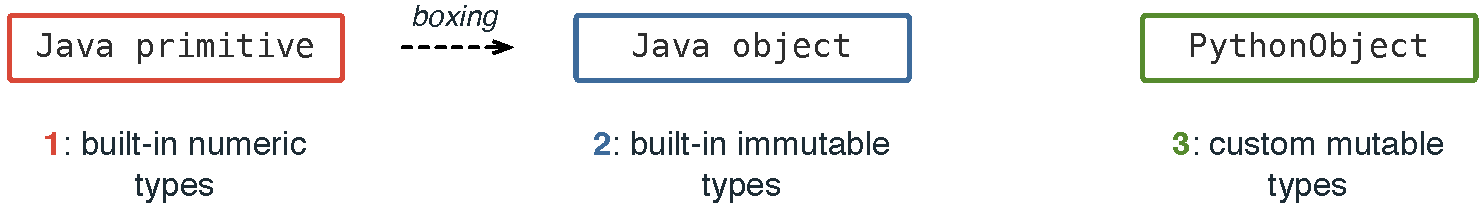
\includegraphics[scale=.34]{figures/three-data-representations}
\caption{Three data representations for Python objects}
\label{fig:three-data-representations}
\end{figure}

Python, although being a dynamic language, has a rich set of built-in types that are backed by C structs.
These types are inherently immutable.
Meaning that Python programs cannot add or remove attributes to or from it at runtime.
This feature separates it from languages like Ruby where you can monkey patch core classes of the language.
But it does offer opportunities for the language implementations like ZipPy to model immutable built-in types in a more efficient way.
Custom types defined in Python level are dynamic and mutable.
They can be as expected manipulated as map or dictionaries at runtime.
In the rest of this Section, we explain how we model them efficiently in ZipPy.

Python does offer more advanced features like metaclasses and attribute access customizations.
They do make the use of the language even more dynamic.
However, in this paper we donot focus on those advanced features.

\subsection{Multiple Data Representations}

ZipPy internally uses multiple data representations to model Python objects.
Figure~\ref{fig:three-data-representations} illustrates this design scheme.
The descriptions of each data representation are as follows:

\begin{enumerate}

\item \textbf{Built-in numeric types}
ZipPy, as explained in Chapter~, models some built-in numeric types, like \texttt{bool}, \texttt{int} and \texttt{float}, using Java primitives.
This approach helps to achieve Java level performance for arithmetic operations in ZipPy.
We refer types that has a Java primitive representation as \emph{unboxable}.
Each \emph{unboxable} numeric type in ZipPy has a corresponding \emph{boxed} representation using Java objects as a fall-back.
As shown in the Figure, a boxing operation will convert an instance of unboxable type, e.g., \texttt{int}, from its Java primitive representation to the boxed one.

\item \textbf{Built-in immutable types}
Similar to Jython, we implement Python built-in types including numeric types as regular Java classes.
In this way we map Python's built-in type hierarchy onto a Java class based type hierarchy.
Unlike custom types, all built-in types in Python are immutable meaning that user program cannot modify the attributes of an instance of a built-in type.
We take advantage of this immutability by modeling Python built-in types directly using Java classes on the JVM.

\item \textbf{Custom mutable types}
All custom or user defined types in Python are mutable.
That includes Python modules, custom type definitions written in Python and instances of custom classes.
We model them using still a regular Java object, an instance of \texttt{PythonObject} in ZipPy, to circumvent the performance overhead incurred by using a hash map.
ZipPy maps Python attribute accesses to field accesses on the \texttt{PythonObject} object.
We support attribute modifications by maintaining an object layout table for each Python object.
The object layout table keeps track of the memory offset for each attribute that is currently stored on the object.
We will discuss how we support attribute modifications on custom types in more detail in Section~.

\end{enumerate}

Although we model Python objects using different physical data representations, our approach preserve the semantics that every data in Python is an object.
ZipPy support object like operations on each of the data representations described above.
What differs our approach to the existing ones is that we do not treat all Python data types in the same way.
We try to pick the most efficient construct offered by the JVM that is suitable for implementing particular types in Python.
To be more specific, modeling Python numbers as Java primitives enables the best arithmetics performance achievable on the JVM.
Using Java object to model Python object brings the opportunity for ZipPy to close the performance gap of object operations between existing implementations of Python and Java.


\subsection{Math Equations}
You may want to display math equations in three distinct styles:
inline, numbered or non-numbered display.  Each of
the three are discussed in the next sections.

\subsubsection{Inline (In-text) Equations}
A formula that appears in the running text is called an
inline or in-text formula.  It is produced by the
\textbf{math} environment, which can be
invoked with the usual \texttt{{\char'134}begin\,\ldots{\char'134}end}
construction or with the short form \texttt{\$\,\ldots\$}. You
can use any of the symbols and structures,
from $\alpha$ to $\omega$, available in
\LaTeX; this section will simply show a
few examples of in-text equations in context. Notice how
this equation:
\begin{math}
  \lim_{n\rightarrow \infty}x=0
\end{math},
set here in in-line math style, looks slightly different when
set in display style.  (See next section).

\subsubsection{Display Equations}
A numbered display equation---one set off by vertical space from the
text and centered horizontally---is produced by the \textbf{equation}
environment. An unnumbered display equation is produced by the
\textbf{displaymath} environment.

Again, in either environment, you can use any of the symbols
and structures available in \LaTeX\@; this section will just
give a couple of examples of display equations in context.
First, consider the equation, shown as an inline equation above:
\begin{equation}
  \lim_{n\rightarrow \infty}x=0
\end{equation}
Notice how it is formatted somewhat differently in
the \textbf{displaymath}
environment.  Now, we'll enter an unnumbered equation:
\begin{displaymath}
  \sum_{i=0}^{\infty} x + 1
\end{displaymath}
and follow it with another numbered equation:
\begin{equation}
  \sum_{i=0}^{\infty}x_i=\int_{0}^{\pi+2} f
\end{equation}
just to demonstrate \LaTeX's able handling of numbering.

\subsection{Citations}
Citations to articles,
conference proceedings or maybe
books listed
in the Bibliography section of your
article will occur throughout the text of your article.
You should use BibTeX to automatically produce this bibliography;
you simply need to insert one of several citation commands with
a key of the item cited in the proper location in
the \texttt{.tex} file.
The key is a short reference you invent to uniquely
identify each work; in this sample document, the key is
the first author's surname and a
word from the title.  This identifying key is included
with each item in the \texttt{.bib} file for your article.

The details of the construction of the \texttt{.bib} file
are beyond the scope of this sample document, but more
information can be found in the \textit{Author's Guide},
and exhaustive details in the \textit{\LaTeX\ User's
Guide} by Lamport.


This article shows only the plainest form
of the citation command, using \texttt{{\char'134}cite}.

\subsection{Tables}
Because tables cannot be split across pages, the best
placement for them is typically the top of the page
nearest their initial cite.  To
ensure this proper ``floating'' placement of tables, use the
environment \textbf{table} to enclose the table's contents and
the table caption.  The contents of the table itself must go
in the \textbf{tabular} environment, to
be aligned properly in rows and columns, with the desired
horizontal and vertical rules.  Again, detailed instructions
on \textbf{tabular} material
are found in the \textit{\LaTeX\ User's Guide}.

Immediately following this sentence is the point at which
Table~\ref{tab:freq} is included in the input file; compare the
placement of the table here with the table in the printed
output of this document.

\begin{table}
  \caption{Frequency of Special Characters}
  \label{tab:freq}
  \begin{tabular}{ccl}
    \toprule
    Non-English or Math&Frequency&Comments\\
    \midrule
    \O & 1 in 1,000& For Swedish names\\
    $\pi$ & 1 in 5& Common in math\\
    \$ & 4 in 5 & Used in business\\
    $\Psi^2_1$ & 1 in 40,000& Unexplained usage\\
  \bottomrule
\end{tabular}
\end{table}

To set a wider table, which takes up the whole width of the page's
live area, use the environment \textbf{table*} to enclose the table's
contents and the table caption.  As with a single-column table, this
wide table will ``float'' to a location deemed more desirable.
Immediately following this sentence is the point at which
Table~\ref{tab:commands} is included in the input file; again, it is
instructive to compare the placement of the table here with the table
in the printed output of this document.


\begin{table*}
  \caption{Some Typical Commands}
  \label{tab:commands}
  \begin{tabular}{ccl}
    \toprule
    Command &A Number & Comments\\
    \midrule
    \texttt{{\char'134}author} & 100& Author \\
    \texttt{{\char'134}table}& 300 & For tables\\
    \texttt{{\char'134}table*}& 400& For wider tables\\
    \bottomrule
  \end{tabular}
\end{table*}
% end the environment with {table*}, NOTE not {table}!

It is strongly recommended to use the package booktabs
and follow its main principles of typography with respect to tables:
\begin{enumerate}
\item Never, ever use vertical rules.
\item Never use double rules.
\end{enumerate}
It is also a good idea not to overuse horizontal rules.


\subsection{Figures}

Like tables, figures cannot be split across pages; the best placement
for them is typically the top or the bottom of the page nearest their
initial cite.  To ensure this proper ``floating'' placement of
figures, use the environment \textbf{figure} to enclose the figure and
its caption.

This sample document contains examples of \texttt{.eps} files to be
displayable with \LaTeX.  If you work with pdf\LaTeX, use files in the
\texttt{.pdf} format.  Note that most modern \TeX\ systems will convert
\texttt{.eps} to \texttt{.pdf} for you on the fly.  More details on
each of these are found in the \textit{Author's Guide}.

\begin{figure}

\includegraphics{fly}
\caption{A sample black and white graphic.}
\end{figure}

\begin{figure}

\includegraphics[height=1in, width=1in]{fly}
\caption{A sample black and white graphic
that has been resized with the \texttt{includegraphics} command.}
\end{figure}


As was the case with tables, you may want a figure that spans two
columns.  To do this, and still to ensure proper ``floating''
placement of tables, use the environment \textbf{figure*} to enclose
the figure and its caption.  And don't forget to end the environment
with \textbf{figure*}, not \textbf{figure}!

\begin{figure*}
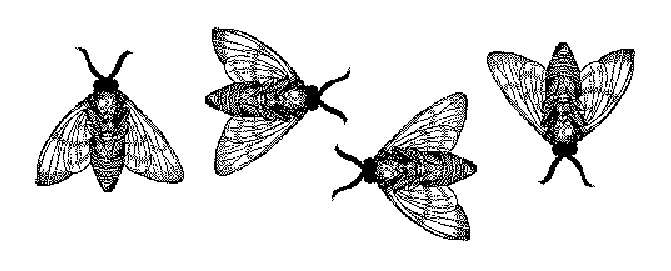
\includegraphics{flies}
\caption{A sample black and white graphic
that needs to span two columns of text.}
\end{figure*}


\begin{figure}
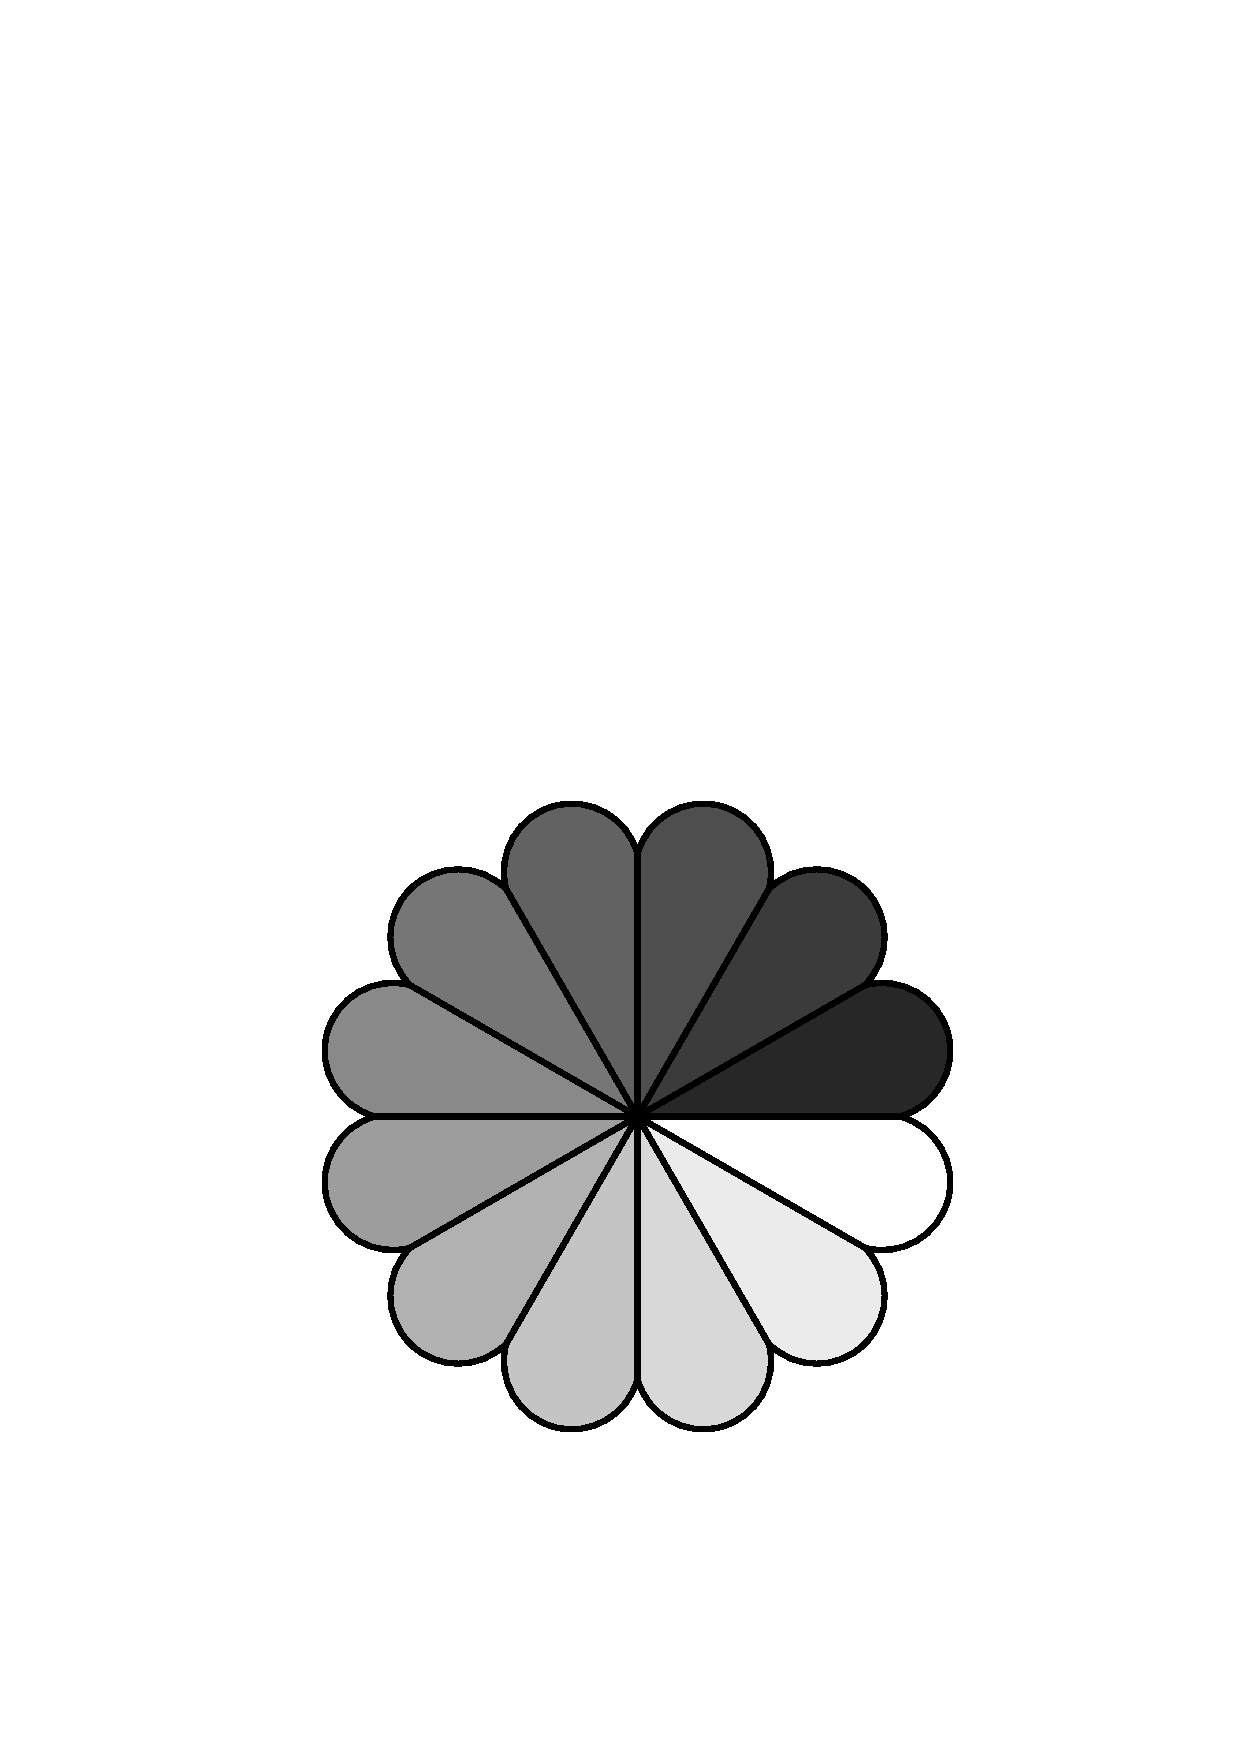
\includegraphics[height=1in, width=1in]{rosette}
\caption{A sample black and white graphic that has
been resized with the \texttt{includegraphics} command.}
\end{figure}

\section{Conclusions}
This paragraph will end the body of this sample document.


\begin{acks}
  The authors would like to thank Dr. Yuhua Li for providing the
  matlab code of  the \textit{BEPS} method. 

  The authors would also like to thank the anonymous referees for
  their valuable comments and helpful suggestions. The work is
  supported by the \grantsponsor{GS501100001809}{National Natural
    Science Foundation of
    China}{http://dx.doi.org/10.13039/501100001809} under Grant
  No.:~\grantnum{GS501100001809}{61273304}
  and~\grantnum[http://www.nnsf.cn/youngscientsts]{GS501100001809}{Young
    Scientsts' Support Program}.

\end{acks}
